%\documentclass[iop]{emulateapj}
\documentclass[aps, prl, twocolumn, nofootinbib, groupedaddress, amsfonts, amssymb, amsmath]{revtex4-1}
\usepackage{graphicx}
\usepackage{bm}
\usepackage{natbib}
%\usepackage[colorlinks=True, linkcolor=blue, citecolor=blue]{hyperref}
%\usepackage[all]{hypcap}

\bibliographystyle{apsrev}

\newcommand{\Div}[1]{\ensuremath{\nabla\cdot\left( #1\right)}}
\newcommand{\angles}[1]{\ensuremath{\left\langle #1 \right\rangle}}
\newcommand{\grad}{\ensuremath{\nabla}}
\newcommand{\RB}{Rayleigh-B\'{e}nard }
\newcommand{\stressT}{\ensuremath{\bm{\bar{\bar{\Pi}}}}}
\newcommand{\lilstressT}{\ensuremath{\bm{\bar{\bar{\sigma}}}}}
\newcommand{\nrho}{\ensuremath{n_{\rho}}}
\newcommand{\approptoinn}[2]{\mathrel{\vcenter{
	\offinterlineskip\halign{\hfil$##$\cr
	#1\propto\cr\noalign{\kern2pt}#1\sim\cr\noalign{\kern-2pt}}}}}

\newcommand{\appropto}{\mathpalette\approptoinn\relax}

\newcommand\mnras{{MNRAS}}%
          % Monthly Notices of the RAS

\begin{document}
%%%%% Create nice title and abstract
\author{Evan H. Anders}
\affiliation{Department of Astrophysical \& Planetary Sciences, University of Colorado -- Boulder}
\affiliation{Laboratory for Atmospheric and Space Physics, Boulder, CO}
\author{Benjamin P. Brown}
\affiliation{Department of Astrophysical \& Planetary Sciences, University of Colorado -- Boulder}
\affiliation{Laboratory for Atmospheric and Space Physics, Boulder, CO}
\title{Convective heat transport in stratified atmospheres at low and high Mach number}

\begin{abstract}
Here we study stratified convection in the context of 
plane-parallel, polytropically stratified atmospheres. 
We hold the density stratification (\nrho) and Prandtl 
number (Pr) constant while varying the
Mach number (Ma) and the Rayleigh number (Ra) to determine 
the behavior of the Nusselt number (Nu), 
which quantifies the efficiency of convective heat transport.
As Ra increases and $\text{Ma} \rightarrow 1$, a scaling 
of Nu $\propto$ Ra$^{0.45}$ is observed.  
As Ra increases to a regime where Ma $\geq 1$,
this scaling gives way to a weaker Nu $\propto$ Ra$^{0.19}$. 
In the regime of Ma $\ll 1$, a consistent
Nu $\propto$ Ra$^{0.31}$ is retrieved,  reminiscent of the 
Nu $\propto$ Ra$^{2/7}$ seen in \RB convection.
\end{abstract}
\maketitle


%%%%% Body of the paper
\section{Introduction}
\refstepcounter{section}
\label{sec:intro}
Convection is essential to heat transport in the cores of high mass stars,
the envelopes of low mass stars, and the atmospheres of terrestrial and 
jovian planets.  The convective dynamics are influenced by the atmospheric 
stratification, which is small in some systems but extends up to 
14 density scale heights in the Sun's convective envelope.
Understanding the fundamental
properties of compressible convection in stratified media is essential
to characterizing systems in astrophysics and planetary sciences.  
Numerical constraints have often restricted studies of compressible
convection to moderately high Mach number (Ma), appropriate to regions near 
the Sun's surface.  Few fundamental properties of the 
low-Ma stratified convection which occurs in the deep solar interior are known.

Early numerical experiments on stratified convection
in two \cite{graham1975, chan&all1982,
hurlburt&all1984, cattaneo&all1990} and three 
\cite{cattaneo&all1991, brummell&all1996} dimensions
revealed a number of basic properties in the moderate-to-high 
Ma regime. In the widely-studied \RB (hereafter RB) problem, 
upflows and downflows are symmetrical and
the temperature gradient approaches zero in the convective interior 
causing the conductive flux to similarly 
disappear.  Highly stratified convection exhibits narrow downflow 
lanes and broad upflow regions.
Furthermore, the \emph{entropy} gradient is negated by convection 
rather than the temperature gradient, such
that in the presence of perfectly efficient convection a significant 
component of the flux is still carried by conduction.

In RB convection, there exist two primary control parameters: 
the Rayleigh number (Ra, the ratio of
buoyant driving to diffusive damping) and the Prandtl number 
(Pr, the ratio of viscous to thermal
diffusivity).  These numbers coupled with the aspect ratio of 
the physical domain and the boundary conditions
determine the dynamics of the convection.  In stratified atmospheres, 
in addition to specifying the equation of state and
fundamental properties of the gas, the two control parameters of 
RB convection are joined by the degree of
stratification across the domain and the characteristic 
Ma of the convective flows.  
Polytropically stratified atmospheres, such as those used in 
early studies, are an ideal extension of
RB convection into the stratified realm as the two additional 
control parameters are directly linked to
basic properties of the atmosphere.  The density stratification is 
set by the number of density scale heights
the atmosphere spans (\nrho), and Ma is controlled 
by the superadiabatic excess ($\epsilon$,
the deviation of the polytropic index from the adiabatic polytropic 
index \cite{graham1975}).

In this letter we study the behavior of convective heat transport, quantified by
the Nusselt number (Nu), in plane-parallel, two-dimensional, polytropically stratified atmospheres.  
$\epsilon$ and Ra are varied  while $\nrho$, Pr, and the aspect ratio are held
constant.  In section 
\ref{sec:experiment}, the construction of atmospheres, equations, and numerical methods are discussed.  
Results are described in section \ref{sec:results} and their implications are discussed
in section \ref{sec:discussion}.

\section{Experiment} 
\refstepcounter{section}
\label{sec:experiment}
In order to compare our results with previous studies and in an effort to examine a simplest case,
we study a fluid composed of monatomic ideal gas particles with an adiabatic index of $\gamma = 5/3$ and
whose equation of state is $P = R\rho T$. In constructing an initial atmosphere, we assume
that the gravitational
acceleration and conductive heat flux do not vary with depth. Both 
the thermal conductivity, $\kappa$, and the temperature gradient, $\grad T_0$, are constant,
such that $\bm{F}_{\text{cond,0}} = -\kappa \grad T_0 = \text{constant}$.
Under these assumptions, satisfying hydrostatic equilibrium produces an atmosphere defined by
\begin{equation}
\begin{split}
\rho_0(z) &= \rho_{t}(z_0 - z)^m \\
T_0(z)    &= T_{t}(z_0 - z).
\label{eqn:polytrope}
\end{split}
\end{equation}
The polytropic index is $m = m_{ad} - \epsilon$
where $m_{ad} \equiv (\gamma-1)^{-1}$ is the adiabatic polytropic index and $\epsilon$ is the
superadiabatic excess.
The subsequent entropy gradient at the top of the atmosphere is $\grad S(L_z) = -\epsilon$. 
Thermodynamic variables are nondimensionalized at the top of the atmosphere as 
$P_0(L_z) = \rho_0(L_z) = T_0(L_z) = 1$, requiring $z_0 \equiv L_z + 1$ and $R = T_{t} = \rho_{t} = 1$.
By this choice, the non-dimensional length scale is the inverse temperature gradient scale and
the timescale is the isothermal sound crossing time of this unit length.
$z$ increases upwards within $[0, L_{z}]$, where $L_{z} = e^{n_{\rho}/m} - 1$ is
determined by the number of density scale heights the atmosphere spans, $n_\rho$.
Throughout this letter, we set $n_{\rho} = 3$ such that the density varies by a factor of 20.
The characteristic timescale of convective dynamics
is related to the atmospheric buoyancy time, $t_{\text{b}} = \sqrt{L_z/g\epsilon}$, with $g = (m+1)$.
We use buoyancy time units in this letter.

Atmospheric diffusivities are specified by the Rayleigh number and the Prandtl number.  The
non-dimensional Rayleigh number is
\begin{equation}
\text{Ra} = \frac{g L_z^3 (\Delta S_0 / c_P)}{\nu\chi},
\end{equation}
where $\Delta S_0$ is the entropy difference between the top and bottom of the atmosphere, 
$c_P = R\gamma(\gamma-1)^{-1}$ is the specific heat at constant pressure,
$\nu$ is the kinematic viscosity (viscous diffusivity), and $\chi$ is the thermal diffusivity.  
The relationship between the thermal and viscous diffusivities is
set by the Prandtl number, Pr$ = \nu/\chi$.   We relate the dynamic viscosity, $\mu$, and the thermal conductivity,
$\kappa$, to their corresponding diffusivities such that 
$\nu \equiv \mu/\rho$ and $\chi \equiv \kappa/\rho$.  As a result, $\text{Ra} \propto (\nu\chi)^{-1} \propto
\rho^2$.  The atmospheres studied here with $n_{\rho} = 3$ experience an increase in the Rayleigh number 
by a factor of 400 across the domain.  This formulation leaves Pr
constant throughout the depth of the atmosphere. In this letter we impose $\text{Pr} = 1$ and
specify Ra at $z = L_z$.  We study atmospheres with an aspect ratio of 4.

At the constant values of $n_\rho$ and Pr used, the primary control parameters of convection are $\epsilon$
and Ra.  We decompose our atmosphere into the background polytrope ($\ln\rho_{0}, T_{0}$) and the fluctuations
about that background ($\bm{u}, \ln\rho_{1}, T_{1}$).  The scaling of the entropy gradient with $\epsilon$
is reflected in the evolved values of these fluctuations, which follow the scaling of
$T_1/T_0 \propto \rho_{1}/\rho_{0} \propto$ Ma$^{2} \propto \epsilon$ for low values of $\epsilon$,
as in Fig. \ref{fig:ma_v_eps}.  

\begin{figure}[t]
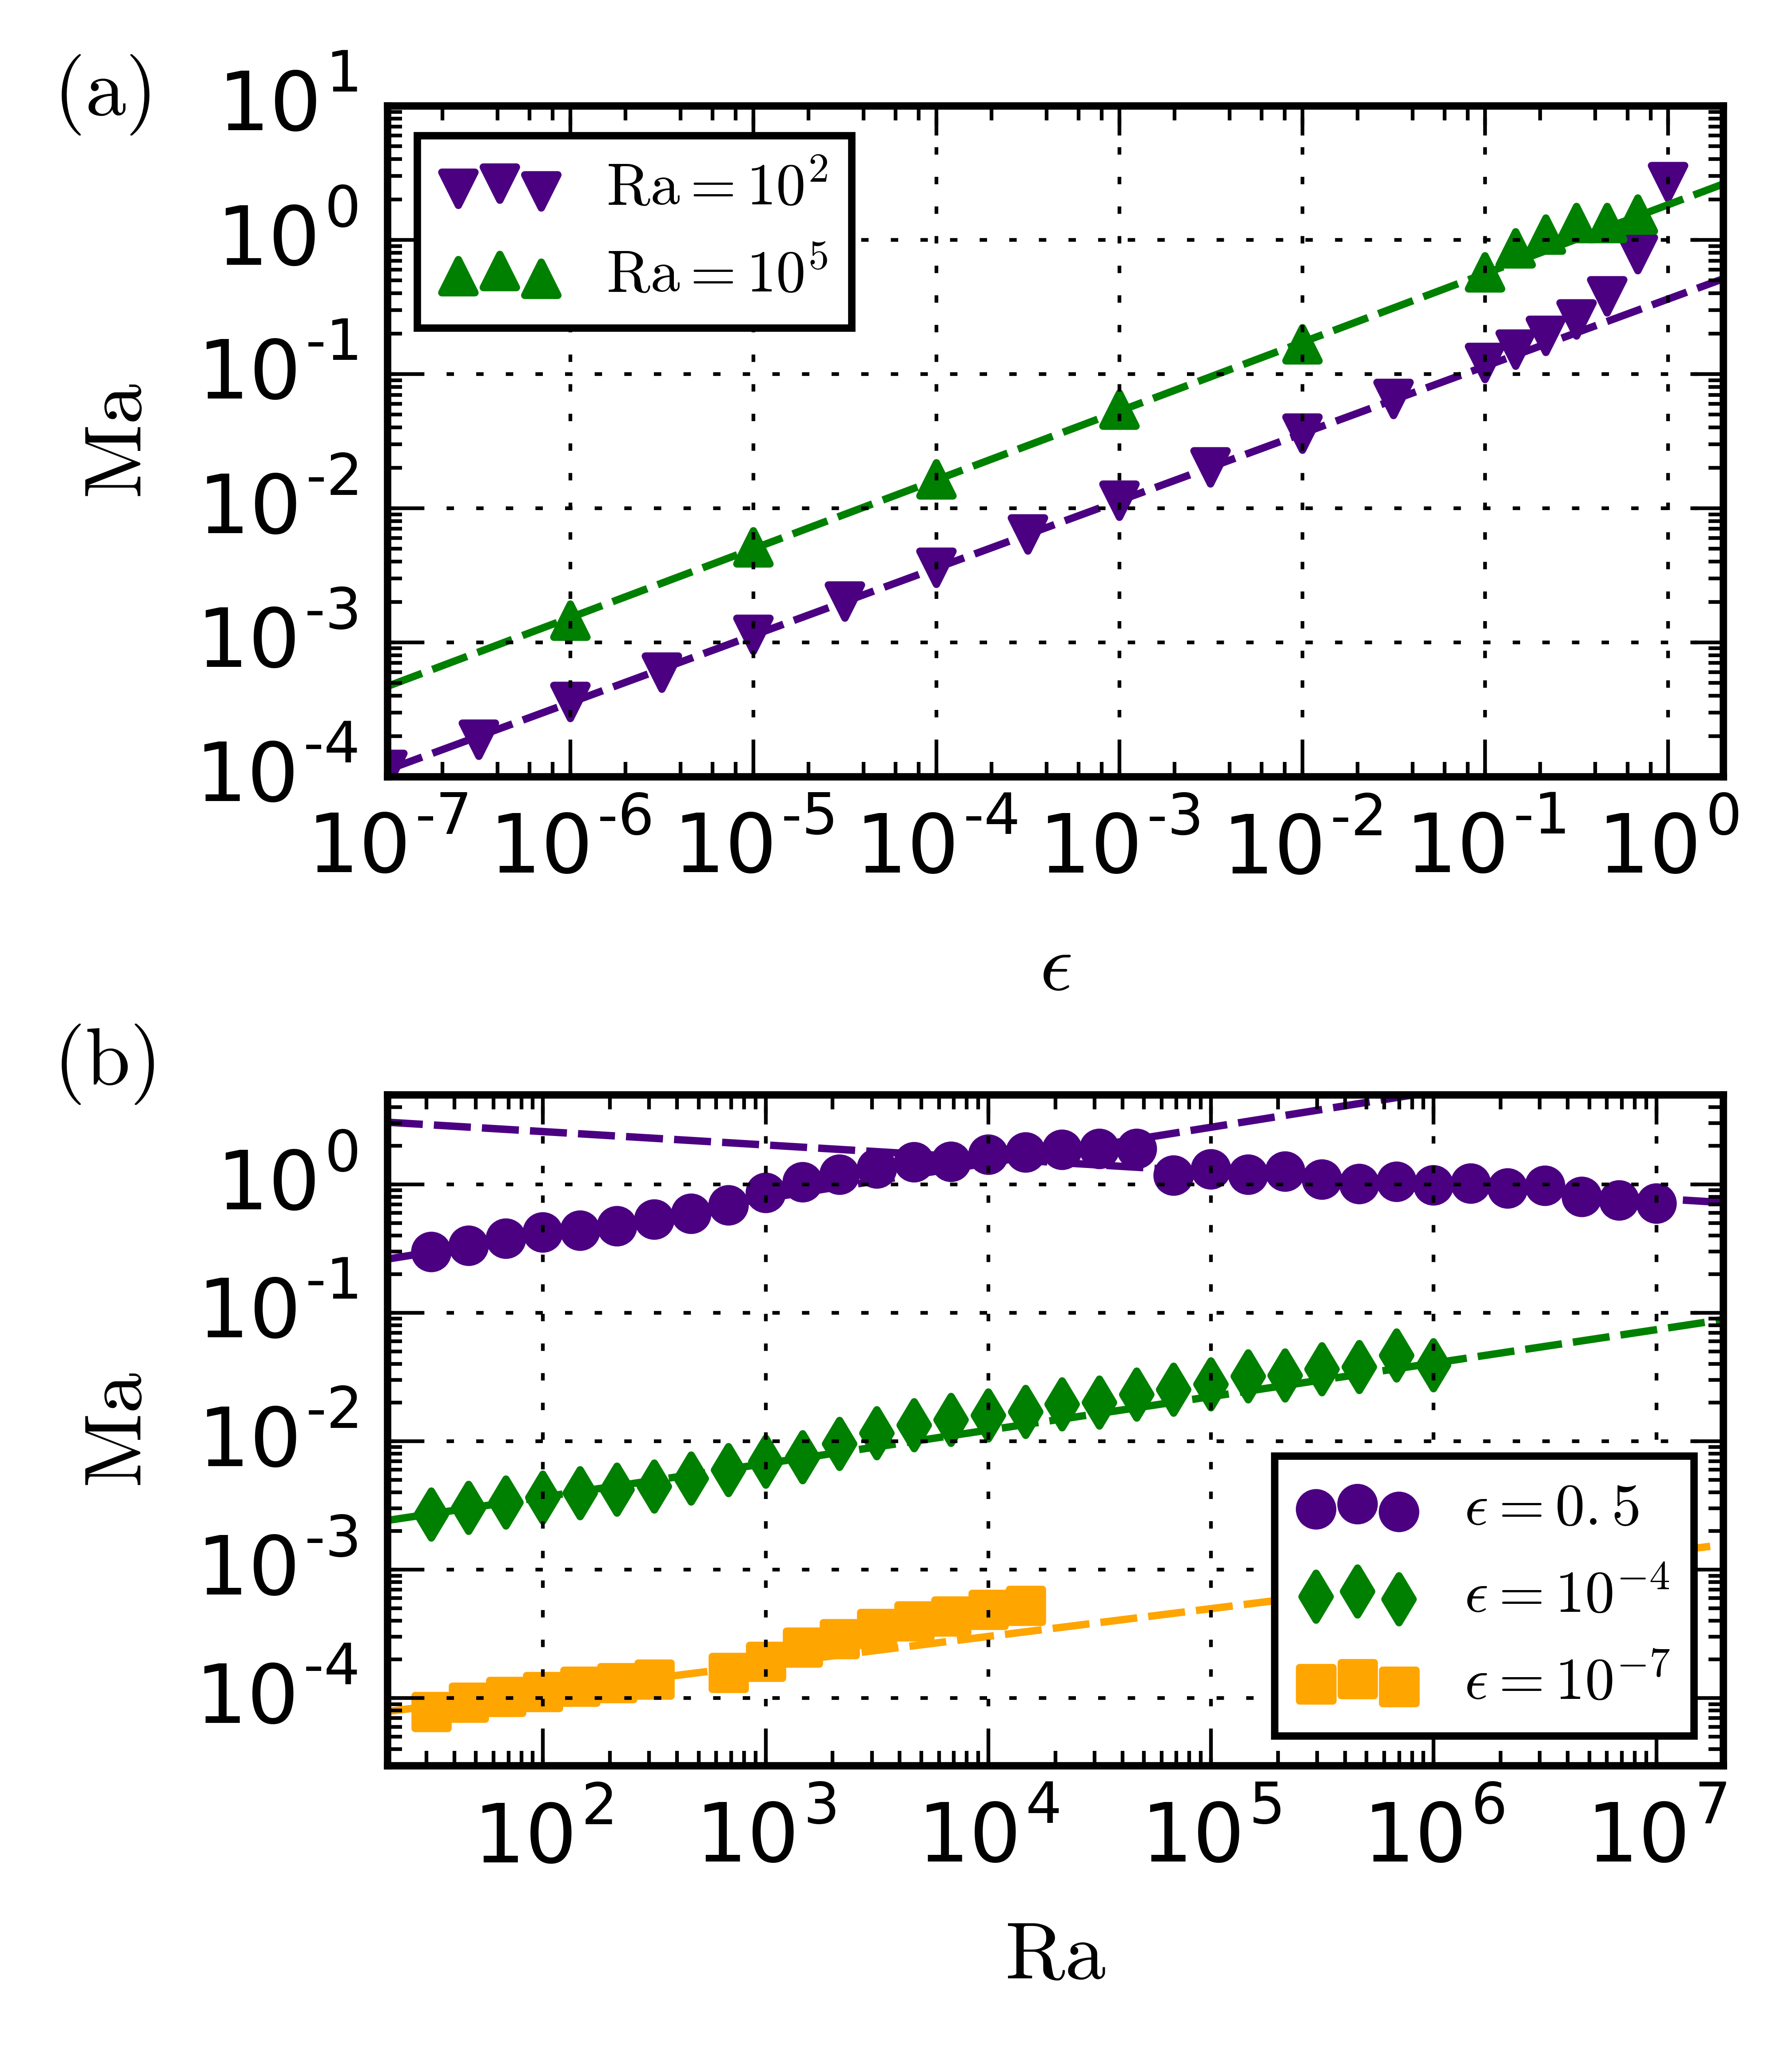
\includegraphics[width=3.4375in]{./figs/ma_v_eps.png}
\caption{The maximum value of Ma which has been horizontally averaged and time averaged for $\geq 100 t_b$, 
beginning roughly $50t_b$ after
the start of simulations.  (a) For $\epsilon \leq 0.1$,
a scaling of $\text{Ma }\propto \{\epsilon^{0.50}, \epsilon^{0.51}\}$ 
at $\text{Ra }= \{10^2, 10^5\}$ exists.
When $\epsilon \rightarrow m_{ad}$, large deviations from this power law are seen.  
(b) At high $\epsilon$, Ma scales as Ra$^{0.28}$ until it reaches the supersonic regime, at which point it
follows a power law of Ra$^{-0.10}$.  At low $\epsilon$, consistent power laws are achieved throughout all
values of Ra studied, where $\text{Ma }\propto \{\text{Ra}^{0.26},\,\text{Ra}^{0.22}\}$
for $\epsilon = \{10^{-4}, 10^{-7}\}$. All
error bars are negligible.  \label{fig:ma_v_eps} }
\end{figure}

The Fully Compressible Navier-Stokes equations,
\begin{align}
&\begin{aligned}
&\frac{\partial \ln\rho}{\partial t} + \Div{\bm{u}} = -\bm{u}\cdot\grad\rho,
	\label{eqn:continuity_eqn}
\end{aligned}\\
&\begin{aligned}
\frac{\partial\bm{u}}{\partial t} + \grad T - &\nu\Div{\lilstressT} - \lilstressT\cdot\grad\nu = \\
&-\bm{u}\cdot\grad\bm{u} - T\grad\ln\rho + \bm{g} + \nu\lilstressT\cdot\grad\ln\rho,
\label{eqn:momentum_eqn}
\end{aligned}\\
&\begin{aligned}
\frac{\partial T}{\partial t} -\frac{1}{c_V}\left(\right.\chi&\left.\grad^2 T + \grad T\cdot\grad\chi\right) = \\
	&-\bm{u}\cdot\grad T - (\gamma-1)T\Div{\bm{u}} \\
	&+ \frac{1}{c_V}\left(\chi\grad T \cdot\grad\ln\rho +\nu\left[\lilstressT\cdot\nabla\right]\cdot\bm{u}\right), 
	\label{eqn:energy_eqn}
\end{aligned}
\end{align}
are evolved with a viscous stress tensor defined as
\begin{equation}
\sigma_{ij} \equiv \left(\frac{\partial u_i}{\partial x_j} + \frac{\partial u_j}{\partial x_i} - \frac{2}{3}\delta_{ij}\Div{\bm{u}}\right).
	\label{eqn:stress_tensor}
\end{equation}
These equations carry a total convective flux of
\begin{equation}
\bm{F}_{\text{conv}} \equiv \bm{F}_{\text{enth}} + \bm{F}_{\text{KE}} + \bm{F}_{\text{PE}} + \bm{F}_{\text{visc}},
\end{equation}
where $\bm{F}_{\text{enth}} \equiv \rho\bm{u}(c_V T + P/\rho)$ is the enthalpy flux, $\bm{F}_{\text{KE}} \equiv 
\rho|\bm{u}|^2\bm{u}/2$ is the kinetic energy flux, $\bm{F}_{\text{PE}} \equiv \rho\bm{u}\phi$ is the potential
energy flux (with $\phi \equiv -gz$), 
and $\bm{F}_{\text{visc}} \equiv -\rho\nu\bm{u}\cdot\lilstressT$ is the viscous flux. 
%Taking an inner product of
%Eq. \ref{eqn:momentum_eqn} with $\bm{u}$ and adding it to 
%Eq. \ref{eqn:energy_eqn}, the full energy equation in conservation form is retrieved,
%\begin{equation}
%\frac{\partial}{\partial t}\left(\rho\left[\frac{|\bm{u}|^2}{2} + c_V T + \phi\right]\right) +
%\Div{\bm{F}_{\text{conv}} + \bm{F}_{\text{cond}}} = 0,
%	\label{eqn:energy_eqn_full}
%\end{equation}
%where $\bm{F}_{\text{cond}} = -\kappa \grad T$.  
Understanding these flux terms and how they interact with the conductive flux, 
$\bm{F}_{\text{cond}} = -\kappa \grad T$, is crucial in characterizing
convective heat transport.

The atmosphere is contained between two impenetrable, stress free, fixed temperature boundaries at
the top and bottom of the domain such that $w = \partial_z u = T_1 = 0$ at $z = \{0, L_z\}$. The domain
is horizontally periodic. We utilize the novel Dedalus\footnote{http://dedalus-project.org/} pseudospectral framework 
 to time-evolve Eqs. 
\ref{eqn:continuity_eqn}-\ref{eqn:energy_eqn} using an implicit-explicit, third-order, four-step 
Runge-Kutta timestepping scheme RK443 \cite{ascher&all1997}.  
Variables are time-evolved on a dealiased Chebyshev (vertical)
and Fourier (horizontal) domain in which the
physical grid dimensions are 3/2 the size of the coefficient grid.  Physical grid sizes range from
96x384 grid points at the lowest values of Ra to 1152x4608 grid points at Ra $\geq 10^{7}$. 
By using IMEX timestepping, we implicitly step the stiff linear acoustic wave contribution and we are able to
efficiently study flows at moderate ($\text{Ma } \approx 1$) and very low ($\text{Ma } \approx 10^{-4}$)
Mach number (Fig. \ref{fig:ma_v_eps}b).  Our equations take the form
of the FC equations in \cite{lecoanet&all2014}, extended to include variable
$\nu$ and $\chi$, and we follow the approach there; this IMEX approach has been successfully 
tested against a nonlinear benchmark  of the compressible Kelvin-Helmholtz instability \cite{Lecoanet_et_al_2016_KH}.

\section{Results}
\refstepcounter{section}
\label{sec:results}

The efficiency of convection is quantified by the Nusselt number.  
Nu is well-defined in RB convection
as total flux normalized by the steady-state background conductive flux 
\cite{johnston&doering2009, otero&all2002}.
In stratified convection Nu is more difficulut to define, but one of the earliest definitions used
was \cite{graham1975,hurlburt&all1984}
\begin{equation}
\text{Nu} \equiv \frac{F_{\text{conv, z}} + F_{\text{cond, z}} - F_{\text{A}}}{F_{\text{ref}} - F_{\text{A}}},
\label{eqn:nusselt}
\end{equation}
where $F_{\text{conv, z}}$ and $F_{\text{cond, z}}$ are the z-components of $\bm{F}_{\text{conv}}$ and $\bm{F}_{\text{cond}}$,
respectively.  $F_{\text{A}} \equiv -\kappa \partial_z T_{\text{ad}}$ is the adiabatic conductive flux, and
$\partial_z T_{\text{ad}} \equiv - g / c_{P}$ for an ideal gas in hydrostatic equilibrium.
$F_{\text{ref}} \equiv \Delta T / L_z$, where $\Delta T \equiv T(L_z) - T(0)$ is the 
conductive flux of a linear profile connecting the upper
and lower plates, which is constant for the choice of fixed-temperature boundaries.

We contend that this is the general form of the Nusselt number and illustrate this with a few limiting
cases. Convection works to
suppress entropy stratification and create isentropic atmospheres.  Under the Boussinesq approximation,
in which density variations are ignored, entropy stratification is directly proportional to temperature stratification,
such that $\grad S \rightarrow 0$ when $\grad T \rightarrow 0$.  Thus, for RB convection, the familiar Nu is
retrieved from Eq. \ref{eqn:nusselt} because $\grad T_{\text{ad}} = 0$.  
In the case of polytropic convection,
as $\epsilon \rightarrow m_{ad} + 1$, $g \rightarrow 0$, so
$\grad T_{\text{ad}} \rightarrow 0$.  In such a case, $F_{\text{A}} \rightarrow 0$ and the
definition of the RB Nu is appropriate to use, as convection carries all of the
flux \cite{brandenburg&all2005}. As $\epsilon \rightarrow 0$, 
$\grad T_{\text{ad}}\rightarrow \grad T_0$, and increasingly
smaller velocity and thermodynamic perturbations are needed to achieve $\grad S = 0$ (Fig. \ref{fig:ma_v_eps}a).
Here, the removal of $F_{\text{A}}$ in the numerator and denominator of Eq. \ref{eqn:nusselt} makes them both
O($\epsilon$), so the overall Nu is sensible.

\begin{figure}[b]
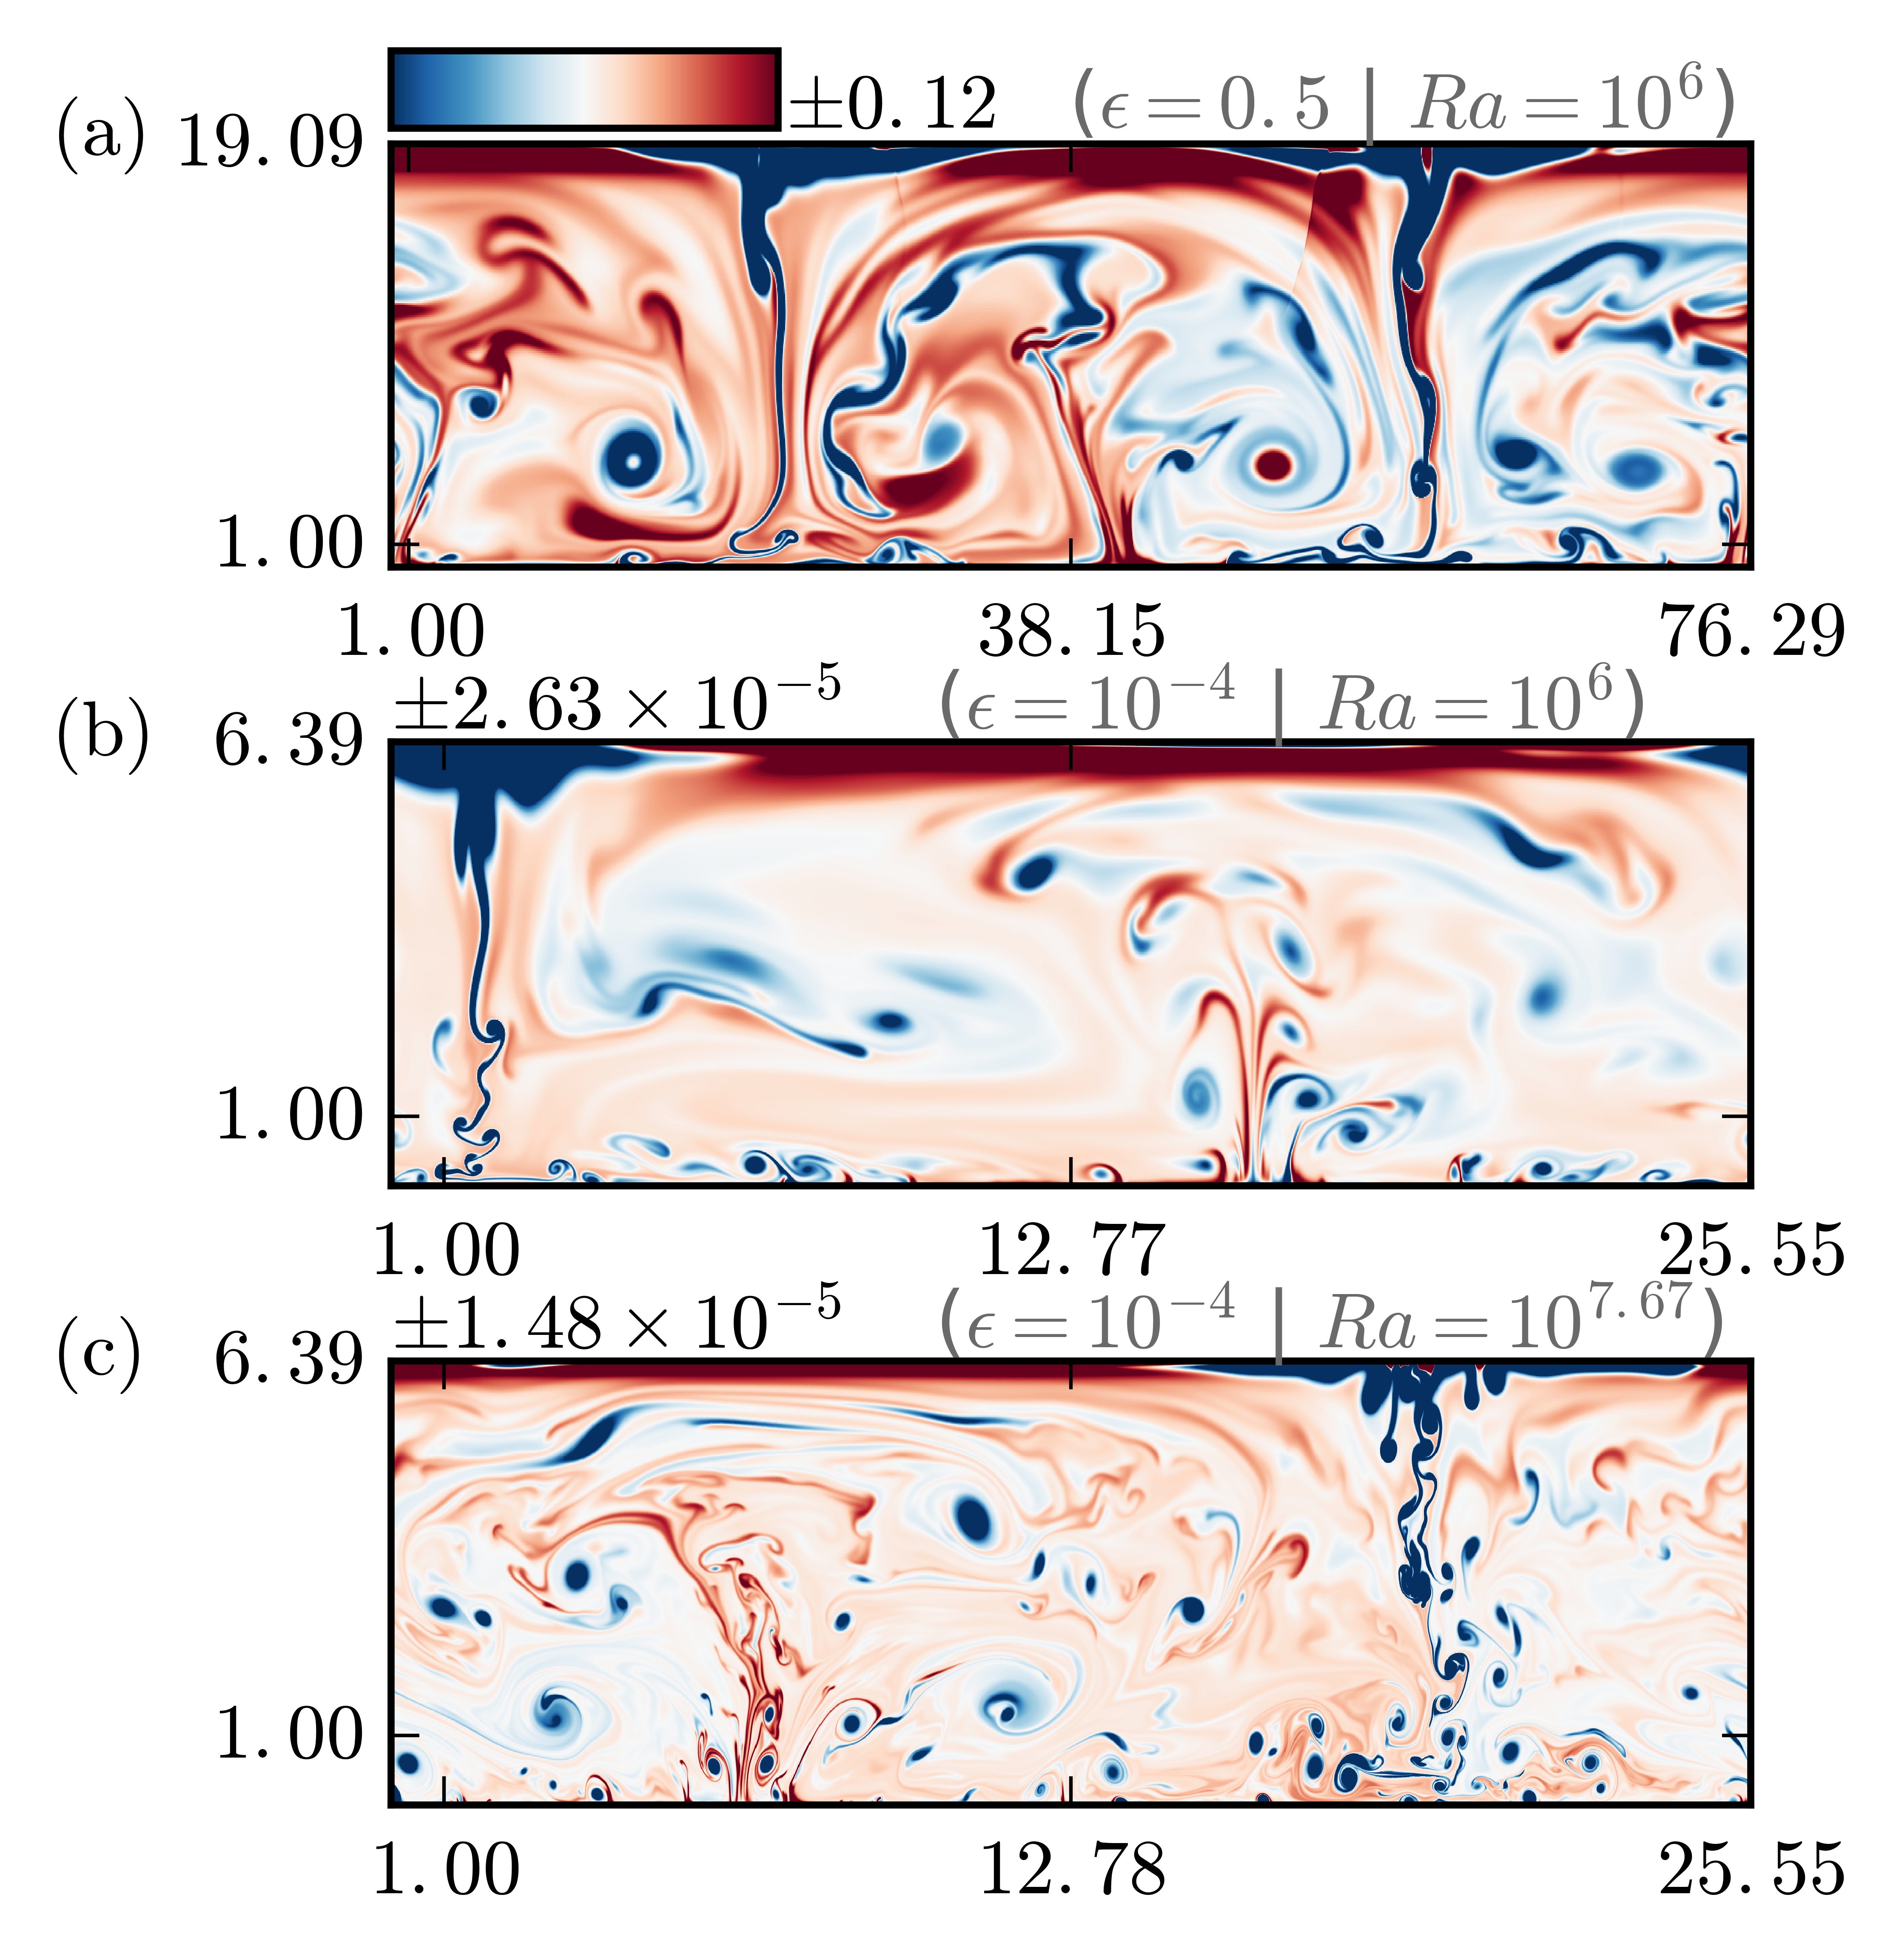
\includegraphics[width=3.4375in]{./figs/snapshots_fig.png}
\caption{Characteristic entropy fluctuations in evolved flows. The time- and horizontally-
averaged profile is removed in all cases.  At high
$\epsilon$ (a), shock systems form near the upper downflow lanes and propel shock-heated material deep within
the atmosphere at sufficiently high Ra.  At low $\epsilon$ but at the same Ra (b), shock systems are absent, 
but otherwise the dynamics are similar.  As Ra is increased (c), downflow lanes no longer span
the entirety of the domain and individual small blobs are responsible for carrying the flux.
\label{fig:entropy_snapshots} }
\end{figure}

Initial value problems were solved in which $T_1$ experienced an infinitesimal kick compared to $\epsilon$
away from hydrostatic and thermal equilibrium.
Solutions were time-evolved until a long average of Nu showed little
dependence on depth. A linear stability analysis determined that the onset of convection
occurs at $\text{Ra}_c = \{10.06, 10.97, 10.97\}$ for $\epsilon = \{0.5, 10^{-4}, 10^{-7}\}$, respectively.  Rayleigh
numbers from values at onset up to nearly $10^6$Ra$_c$ for $\epsilon = 0.5$, $10^5$Ra$_c$ for $\epsilon = 10^{-4}$,
and $10^3$Ra$_c$ for $\epsilon = 10^{-7}$ were studied.  

At large $\epsilon$ (0.5), shock systems form in the upper atmosphere near downflow lanes 
(Fig. \ref{fig:entropy_snapshots}a) and propagate toward upflow lanes.  
Such systems were reported in
both two \cite{cattaneo&all1990} and three \cite{malagoli&all1990} dimensional polytropic simulations previously.
These shocks heat material entering the downflows, reducing both the
buoyant driving and the efficiency of convective transport.

Low Mach number flows, such as those in an $\epsilon = 10^{-4}$ atmosphere (Fig. \ref{fig:entropy_snapshots}b)
have similar bulk thermodynamic structure but lack the complicating dynamics of shock heating. 
Low Ma flows are in pressure equilibrium with their suroundings, so
pressure forces are unlikely to be the sole cause of symmetry breaking in up- and downflows, as has been suggested
\cite{hurlburt&all1984};  it is more likely that these flows are responding to 
the effects of density stratification.
As Ra is increased to large values (Fig. \ref{fig:entropy_snapshots}c), thermodynamic structures 
no longer span the whole domain but rather break up into small packets which traverse the domain multiple
times before diffusing.  
The complicated nature of high Ra dynamics, especially in the low Ma regime,
has prevented the convergence of solutions in the regime of 
$\text{Ra }> 10^5\text{Ra}_c$ at low $\epsilon$.

\begin{figure}[t]
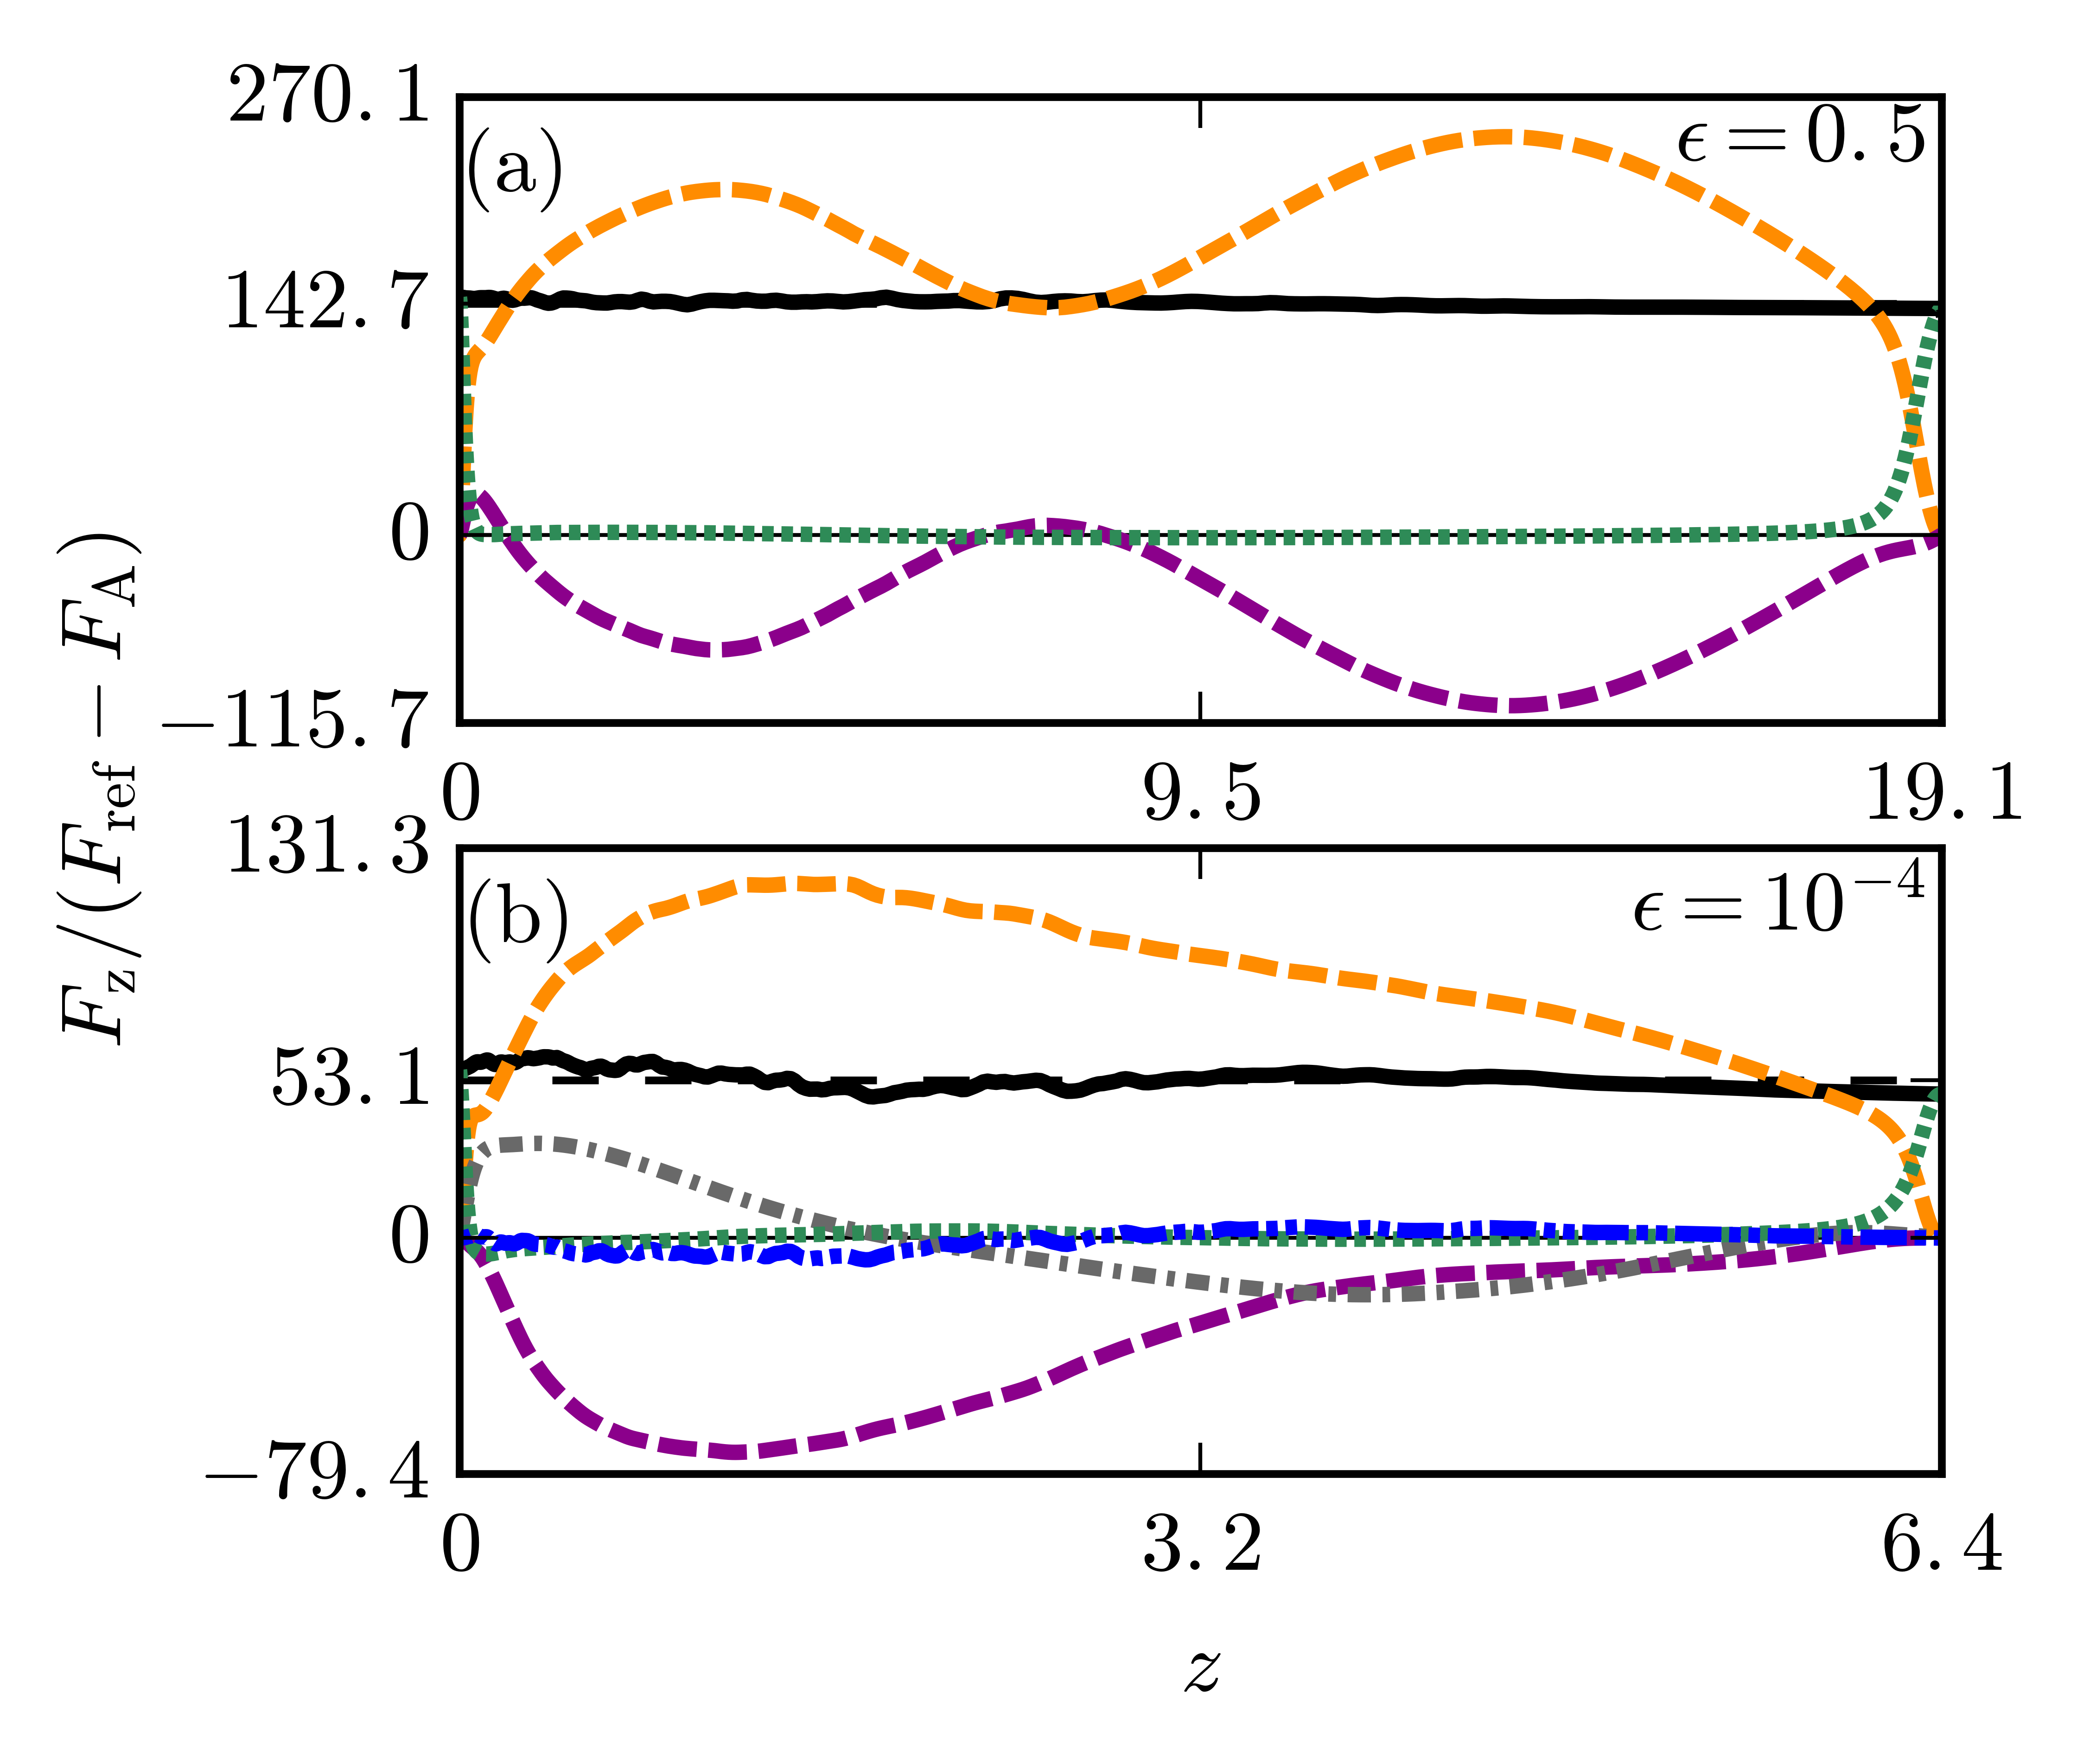
\includegraphics[width=3.4375in]{./figs/fluxes_fig.png}
\caption{Time-averaged flux profiles for high (top) and low (bottom) Ma flows at $\text{Ra }= 10^6$.  
The dashed lines correspond to the
enthalpy flux (orange, positive) and kinetic energy flux (purple, negative).  The grey dash-dot line is the
viscous flux, the blue dash-dot-dot line is the potential energy flux, 
and the green dotted line is the radiative flux with the adiabatic radiative flux removed. All
fluxes are normalized by $F_{\text{ref}} - F_{\text{A}}$, as in Eq. \ref{eqn:nusselt}.  The solid black line is
Nu, the properly normalized sum of all the fluxes \label{fig:flux_profiles} }
\end{figure}

At large Ra, the heat transport properties of the systems become increasingly complex and time-dependent.
Large $\epsilon$ flows exhibit two local maxima in the enthalpy flux and kinetic energy flux: one in the upper 
atmosphere caused by the shocks, and one in the lower atmosphere caused by the deep mixing of convective motions
(Fig. \ref{fig:flux_profiles}a).
At low $\epsilon$, only the deep maximum is present (Fig. \ref{fig:flux_profiles}b).  
Fixed-temperature boundary conditions allow the flux at the boundaries to vary, so many runs at $\text{Ra }> 10^5$
and $\epsilon = 10^{-4}$ exhibit states in which the flux entering the system at the bottom of the atmosphere 
exceeds that which leaves at the top.  
These states are punctuated by states of vigorous shearing, similar to those previously
reported in two-dimensional RB convection \cite{goluskin&all2014}.  These shearing states push the bottom temperature
gradient towards adiabatic, allowing the excess energy to exit through the upper boundary.  These shearing
states will be covered in more detail in a future paper.  Regardless, a proper long-term average over shearing
and non-shearing states retrieves an invariant flux (and Nu) profile throughout the depth
of the atmosphere. 

After appropriately time-averaging the fluxes, a sensible Nu is retrieved.  Nusselt numbers for
all simulations at low and high Ma are plotted in Fig. \ref{fig:nu_v_ra}.  At $\epsilon = \{10^{-4}, 10^{-7}\}$,
scaling laws of $Nu \propto Nu^{\{0.31, 0.31\}}$ are retrieved.  At $\epsilon = 0.5$, in the near-sonic
regime ($Ra \leq 10^4$), the scaling of $Nu$ with $Ra$ is inflated, with $Nu \propto Ra^{0.45}$.  As simulations
pass into the supersonic regime and shocks start to form near the downflows,
that scaling drops to $Nu \propto Ra^{0.19}$.  Error on all power law scalings is negligible.

\begin{figure}[t]
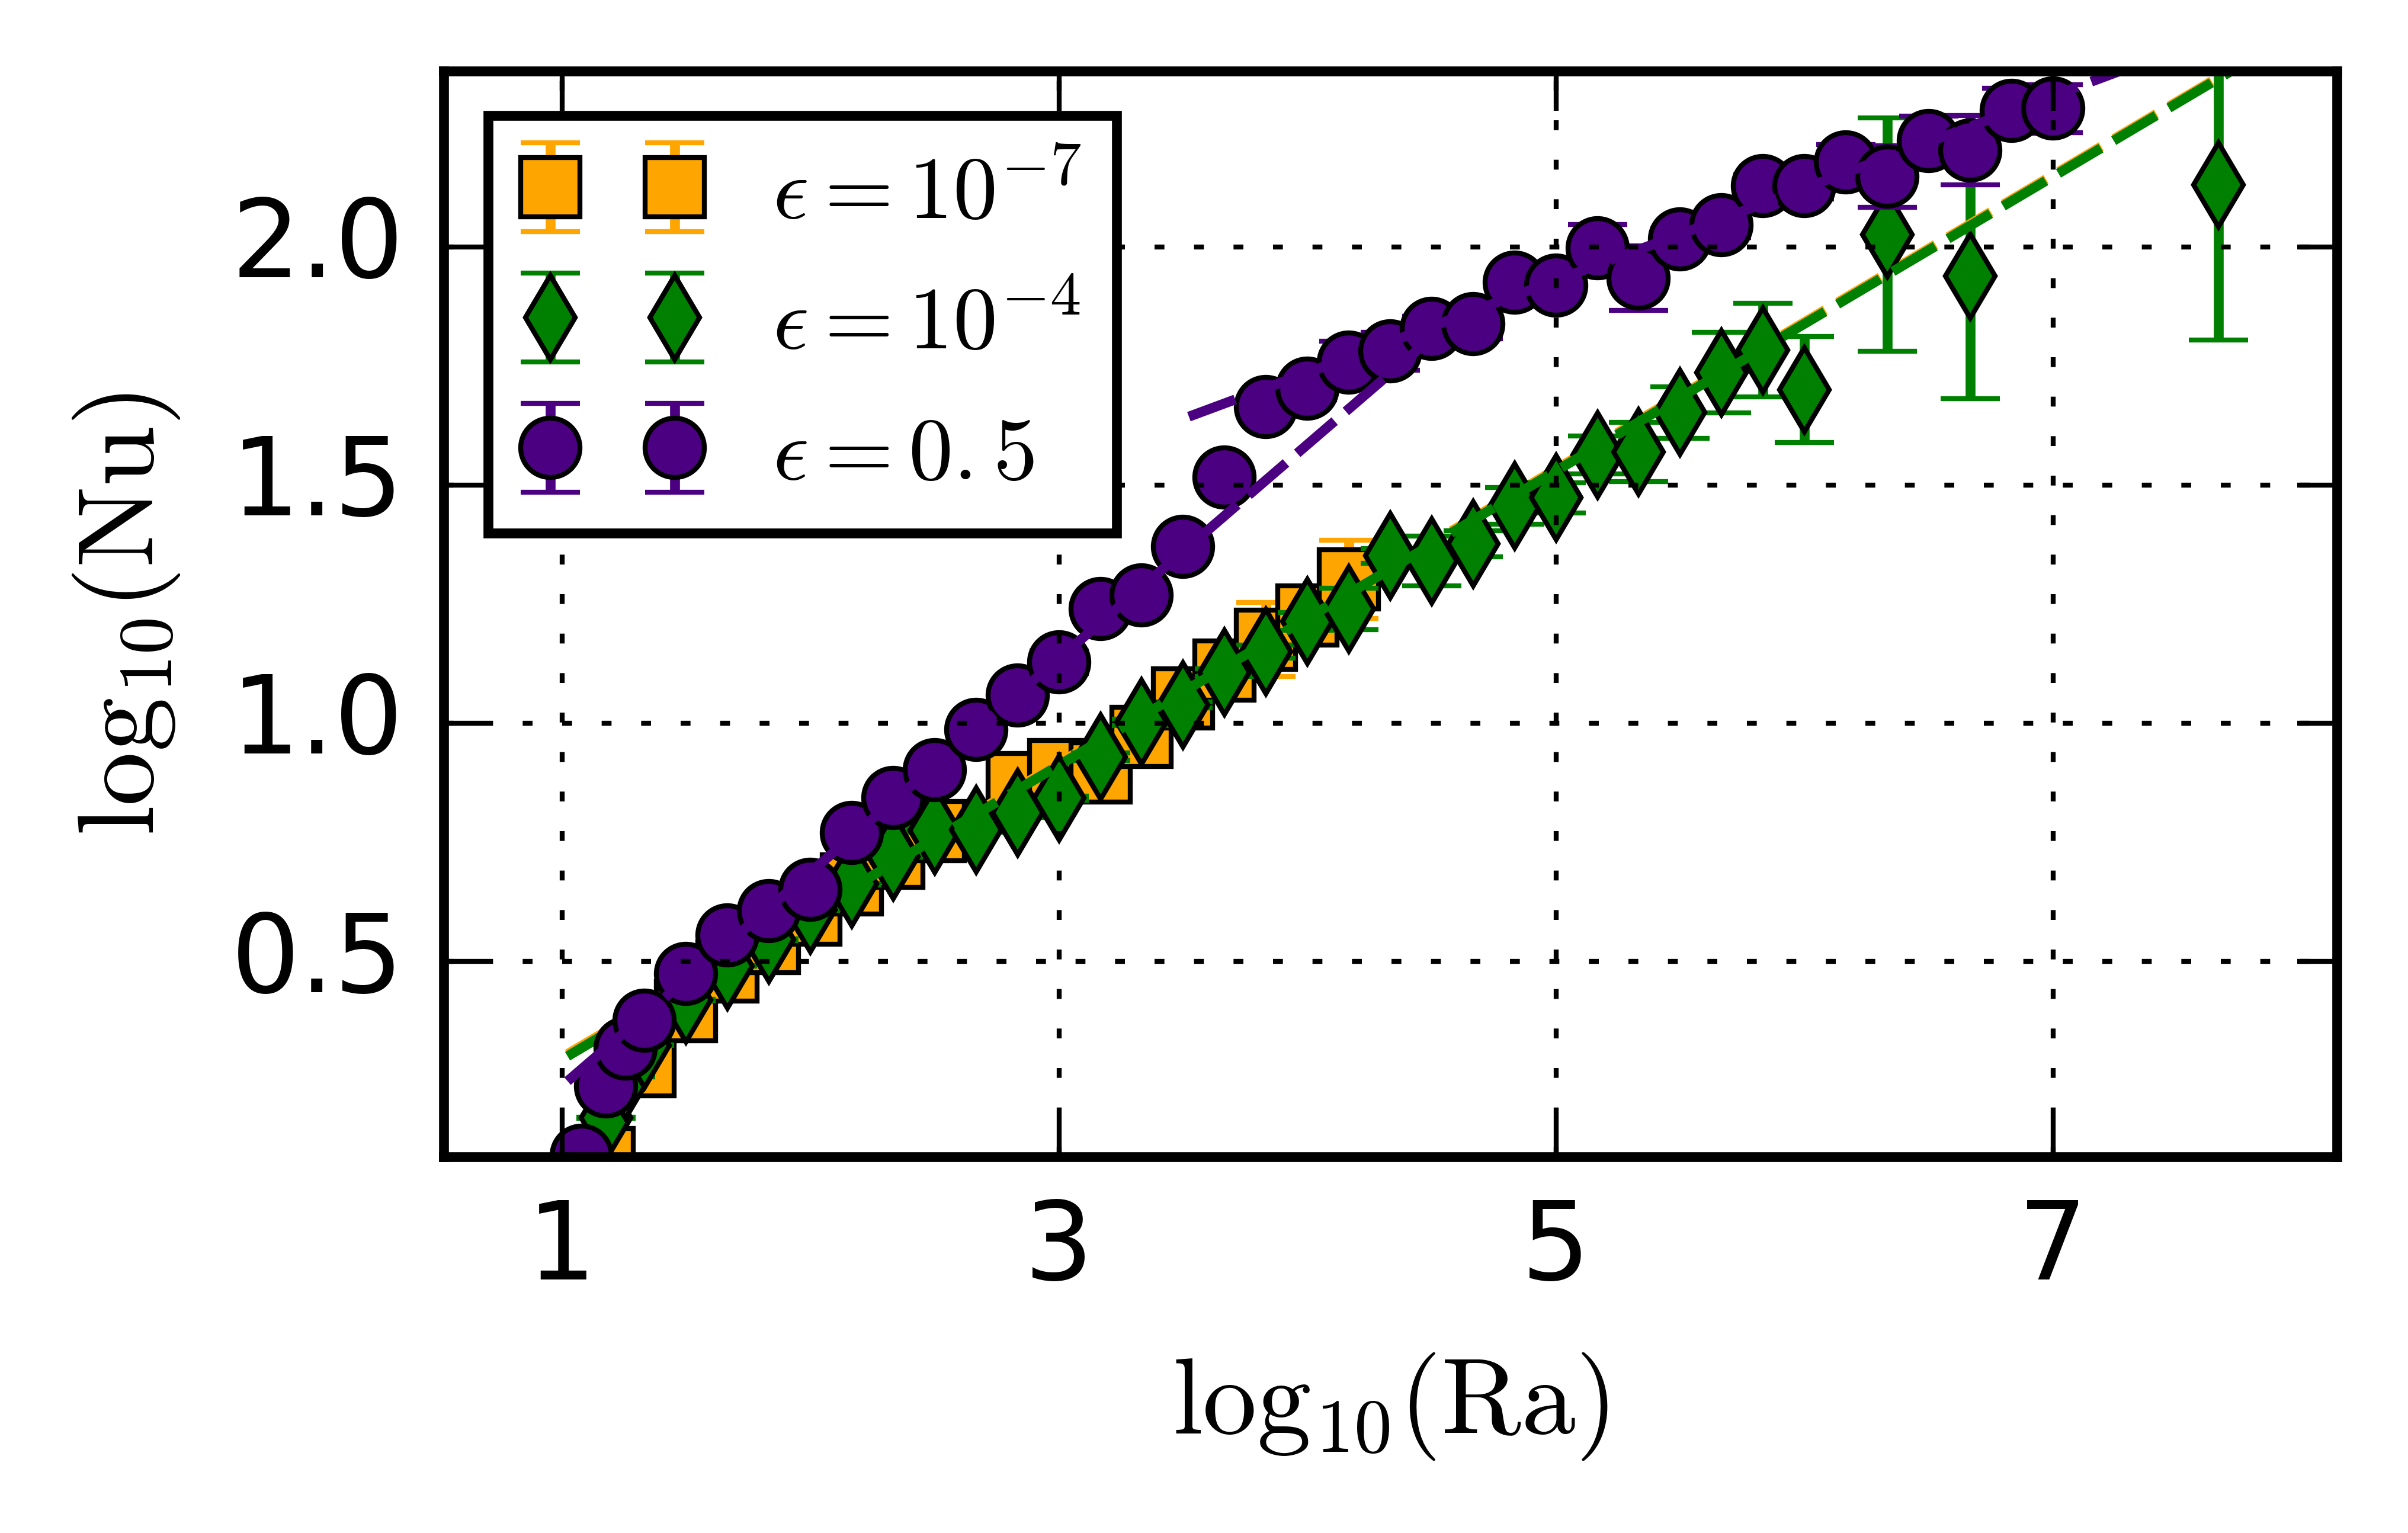
\includegraphics[width=3.4375in]{./figs/nu_v_ra.png}
\caption{Variation of Nu as Ra increases at low and high Ma. 
At high $\epsilon$, a clear transition from the subsonic to supersonic regime is evident in the scaling
of Nu with Ra.  In the low $\epsilon$ regime, Nu scalings collapse onto a similar line which is
reminiscent of RB scalings \cite{johnston&doering2009}.  Error bars represent the square root of
the variance of Nu with depth.
\label{fig:nu_v_ra} }
\end{figure}

\section{Discussion}
\refstepcounter{section}
\label{sec:discussion}
In this letter we have studied fundamental heat transport by stratified convection in simplified 2-D polytropic
atmospheres which are specified by two parameters, $\nrho$ 
and $\epsilon$.  We argue that these atmospheres are the natural extension
of the RB problem to stratified systems, and should be used to understand the basic properties of stratified
convection.  The similarity between the scaling of Nu in RB convection and in low-$\epsilon$ polytropes suggests 
that a boundary layer theory such as the Grossmann-Lohse theory for incompressible flows
could be developed for fully compressible convection in these systems \cite{ahlers&all2009}.  

%Furthermore, we have demonstrated that low Ma flows exhibit the same pattern of broad upflows and narrow downflows
%observed in high Ma flows \cite{hurlburt&all1984}.  At low Ma, flows are often in pressure equilibrium
%with their surroundings, so cooling parcels increases their density, and both of these effects reduce
%entropy.  Neither of the two free thermodynamic variables can cause breaking in warm upflow regions, 
%so stratification effects must cause the observed flow asymmetry.
%While not studied in this work, it is possible that at low Ma, flows feel the pressure response of the
%boundaries, causing deflection in a manner unseen at high Ma.

The dynamics of these polytropic solutions are complex and highly time-dependent, even in two dimensions.
Time-dependent oscillating shear states have developed spontaneously, as seen before in RB convection
\cite{goluskin&all2014}.  While computationally difficult, the highest values of Ra and the lowest value
of $\epsilon$ studied here are far from values found in nature.  If the scalings of Nu and Ma
presented here (Figs. \ref{fig:ma_v_eps} \& \ref{fig:nu_v_ra}) hold, then under solar conditions ($\text{Ra }\approx 10^{20}$, $\text{Ma }\approx 10^{-4}$), we expect that $\epsilon \approx 10^{-20}$ and
$\text{Nu }\approx 10^{6}$.  
Solar conditions are of course more complicated, as there $\kappa$ is
set by the radiative opacity, which depends on both $\rho$ and $T$.

Future work will aim to better understand the mechanisms of shearing states and
whether or not these states are attainable in three-dimensional, non-rotating atmospheres.  Our studies
here have set the groundwork for understanding and comparing heat transport in stratified convection
to that in RB convection \cite{johnston&doering2009}, and for future studies of transport in stratified
convection in more realistic systems, such as those bounded by stable regions \cite{hurlburt&all1986} or 
using more realistic profiles of $\kappa$.



\subsection{acknowledgements}
This work was supported by the CU/NSO George Ellery Hale Graduate Fellowship
and supported by NASA LWS grant number NNX16AC92G.  Computations were conducted 
with support by the NASA High End Computing (HEC) Program through the NASA 
Advanced Supercomputing (NAS) Division at Ames Research Center
with allocations (GID s1647, PI Brown; GID g26133, PI Toomre).
We thank Axel Brandenburg, Mark Rast, and Jeff Oishi for many useful discussions.

\bibliography{../biblio.bib}
\end{document}
